%\section{Motivation}
\subsection{Motivating Scenario}
\label{sec:motivation}

\begin{figure*}[ht]
  \begin{center}
%    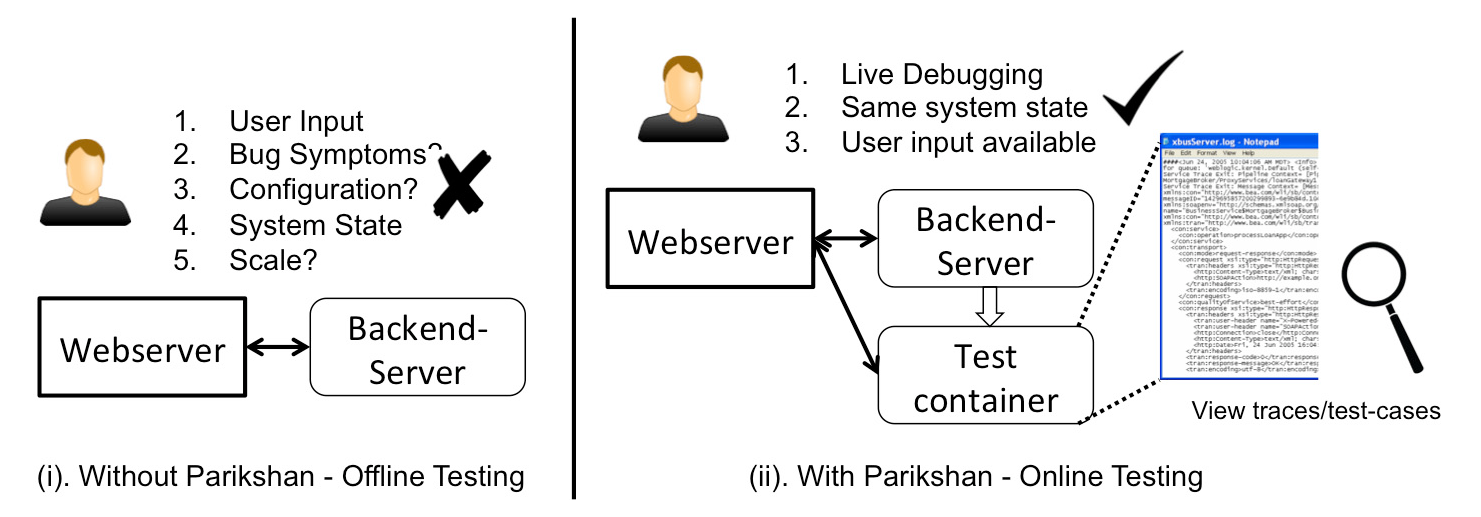
\includegraphics[width=0.7\textwidth]{figs/motivation.eps}
    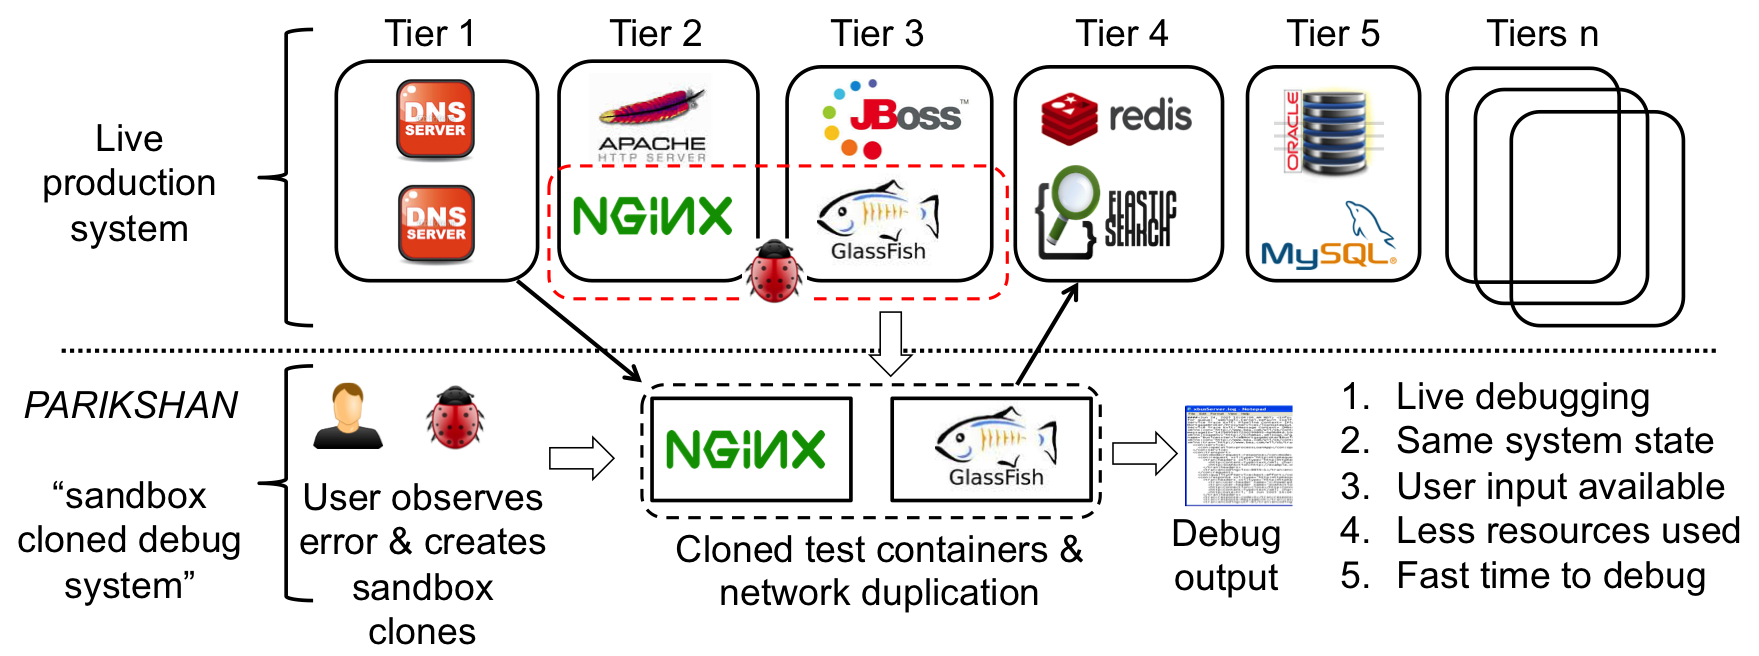
\includegraphics[width=0.99\textwidth]{figs/workflow3.png}
    \caption{Workflow of \parikshan in a live multi-tier production system with several interacting services. When the admin of the system observes errors in two of it's tiers, he can create a sandboxed clone of these tiers and observe/debug them in a sandbox environment without impacting the actual production system.}
    \label{fig:motivation}
  \end{center}
\end{figure*}

%In figure \ref{fig:motivation} 
%In Figure \ref{fig:motivation}, we have shown two workflows of the same system running with \parikshan, and without \parikshan.
To further explain, let us take  user Joe who is an administrator, and IT manager for a multi-tiered system. 
Much like several IT systems user Joe has a dashboard which informs him of the health status of all of his applications, and provides him with high level statistical views of all tiers of the system.
Joe observes an unusually high memory usage in his glassfish server for transaction type X and anomalous error logs in associated nginx systems.
Under usual circumstances, the system would have to go down(depending on the severity of the problem), the problem debugged using offline testing,  and the system would be patched once the problem has been diagnosed.
However often, it is difficult to find out the configuration of the system, and the user input which is causing this problem.
In case of modern large scale systems some errors may happen only at scale, and would require a large test-cluster to recreate the error.
Furthermore, taking down the glassfish and nginx servers would impact several more services otherwise are running fine. 

Joe can now use \parikshan, to fork off a clone of nginx container as \textbf{\textit{nginx-debug}}, and glassfish as \textbf{\textit{glassfish-debug}} container. 
Our proxy network duplication sends a copy of the incoming request to the debug containers, while users can continue using nginx and glassfish services. 
The processes in debug containers follow the same execution paths, as they receive the same input as the production containers.
This allows Joe to initiate deeper traces, and observe the execution without fearing any problems in the user-facing operations.
Time to bug resolution is usually a very important criteria in any user-facing service oriented application.
\parikshan greatly reduces debugging time, and makes capturing the context of the application much easier.

% This paragraph needs serious revision - the points have been noted down but they need to be stated clearly in a better manner.
%One of the key advantages of such an online approach is a reduced time to bug resolution. 
%Time to bug resolution is usually a very important criteria in any user-facing service oriented application, as the longer a bug remains the system, the more it is going to hit the user perception/revenue.
%Bearing this in my mind we believe, that online testing will be an important aspect towards modern applications.
%Additionally the usage of redundant computing for testing in A/B testing(see section \ref{sec:related}) approaches is a well accepted paradigm in real-world applications.
%This leads us to believe that using redundant computing will be acceptable for regular testing approaches as well.
%Using \parikshan is also a way to avoid creating a large test-cluster to do debugging. 

\iffalse
\subsection{Motivation Questions?}

To further motivate our testing paradigm we have come up with a set of motivating questions:

%\begin{compactitem}
%\setlength{\itemsep}{1Pt}
%\item[]\textbf{Q1:} Is it important to sandbox test-cases?
%\item[]\textbf{Q2:} Is recreating production environment difficult? 
%\item[]\textbf{Q3:} Is redundant computing available? 
%\item[]\textbf{Q4:} How would executing test-cases in a production server effect user-experience?
%\end{compactitem}

\subsubsection{\textbf{Q1:} Is it persistent testing important?}
\subsubsection{\textbf{Q2:} Is recreating production environment difficult?}
\subsubsection{\textbf{Q3:} Can redundant computing be utilized for testing?}
\subsubsection{\textbf{Q4:} How would executing test-cases in a production server effect user-experience?}
\fi